% First argument to \section is the title that will go in the table of contents. Second argument is the title that will be printed on the page.
\section[Chương 1]{Chương 1: Điện trường}

\subsection[Câu 1]{Câu 1: Trình bày khái niệm điện trường. Nêu định nghĩa và ý nghĩa của vector cường độ điện trường. Thiết lập công thức xác định vectơ cường độ điện trường gây bởi điện tích điểm, hệ điện tích điểm và của một vật mang điện.}

\begin{itemize}
  \item Điện trường là loại môi trường đặc biệt được tạo ra xung quanh các hạt mang điện tích, có tính chất gây lực tác dụng lên các điện tích đặt trong nó
  \item Vecto cường độ điện trường tại 1 điểm là đại lượng có giá trị bằng lực tác dụng của điện trường lên một đơn vị điện tích dương tại điểm đó
  \begin{itemize}
    \item Vecto cddt gây bởi 1 điện tích điểm: $\vec{E} = \frac{\vec{F}}{q_0} = \frac{q}{4\pi\epsilon_0\epsilon r^3} \vec{r}$
    \item Vecto cddt gây bởi 1 hệ điện tích điểm: $\vec{E} = \frac{\vec{F}}{q_0} = \frac{\sum\limits \vec{F}_i}{q_0} = \sum\limits \frac{\vec{F}_i}{q_0} = \sum\limits \vec{E}_i \Rightarrow$ Nguyên lý chồng chất điện trường
    \item Vecto cddt gây bởi 1 vật mang điện: Chia nhỏ vật thành các phần nhở chứa điện tích $dq$. Coi vật như một hệ vô số điện tích điểm: $\vec{E} = \int d\vec{E} = \int \frac{dq}{4\pi\epsilon_0\epsilon r^2} \frac{\vec{r}}{r}$
  \end{itemize}
\end{itemize}

\subsection[Câu 2]{Câu 2: Định nghĩa đường cảm ứng điện. Cho biết sự khác nhau cơ bản giữa phổ đường sức điện trường và phổ đường cảm ứng điện. Viết công thức xác định thông lượng cảm ứng điện qua diện tích $S$. Tính điện thông qua một mặt cầu bao quanh một điện tích điểm.} 

\begin{itemize}
  \item Đường cảm ứng điện là đường cong mà tiếp tuyến tại mỗi điểm trùng với phương của vecto cảm ứng điện tại điểm đó, chiều của đường cảm ứng điện là chiều của $\vec{D}$.
  \item ĐIểm khác nhau: Đường sức điện trường biểu diễn cho $\vec{E}$, đường cảm ứng điện biểu diễn cho $\vec{D} \Rightarrow$ Đường cảm ứng điện đi qua mặt phân cách các môi trường là đường liên tục
\begin{figure}[h]
  \centering
  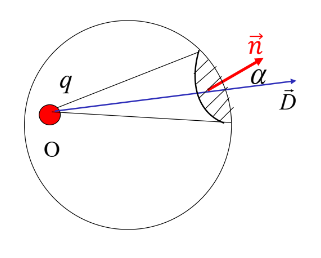
\includegraphics[width=0.5\textwidth]{ch01.png}
\end{figure}
  \item Thông lượng cảm ứng qua diện tích $S$:
  \begin{itemize}
    \item Giả sử diện tích $S$ trong 1 điện trường $\vec{D}$. Chia nhỏ $S$ thành các phần $dS$ sao cho $\vec{D}$ tại mỗi điểm trên $dS$ là như nhau
    \item $d\Phi = \vec{D}d\vec{S} = DdS\cos\alpha = DdS_n \Rightarrow \Phi = \int_S d\Phi = \int_S \vec{D}d\vec{S}$
  \end{itemize}
  \item Góc khối $d\Omega = \frac{dS\cos\alpha}{r^2}$, điện thông qua 1 mặt $d\Phi = \vec{D}d\vec{S} = \frac{q}{4\pi r^3} \vec{r}d\vec{S} = \frac{q}{4\pi} \frac{dS\cos\alpha}{r^2} = \frac{q}{4\pi} d\Omega$
  \item Điện thông qua 1 mặt bao quanh $q$: $\Phi = \oint_S d\Phi = q$
\end{itemize}

\subsection[Câu 3]{Câu 3: Nêu định nghĩa và ý nghĩa của mômen lưỡng cực điện. Xác định vector cường độ điện trường gây bởi lưỡng cực điện tại điểm $M$ nằm trên đường trung trực và cách tâm $O$ của lưỡng cực một khoảng $r$ khá lớn so với khoảng cách giữa hai điện tích.}

\begin{itemize}
  \item Lưỡng cực điện là 1 hệ 2 điện tích điểm bằng nhau về trị số nhưng trái dấu, cách nhau 1 khoảng rất nhỏ so với khoảng cách tới các điểm ta xét
  \item Momen lưỡng cực điện $\vec{p}_e = q\vec{l}$ 
  \item Ý nghĩa: Biết được $\vec{p}_e$ có thể biết được $\vec{E}$ do lưỡng cực điện gây ra. Vậy ta nói $\vec{p}_e$ đặc trưng cho tính chất điện của lưỡng cực
  \item Xác định $E$ tại điểm $M$ nằm trên trung trực và cách xa 2 điểm 1 khoảng $r$ (tự làm)
\end{itemize}

\begin{equation*}
  \vec{E}_m = - \frac{\vec{p}_e}{4\pi\epsilon_0\epsilon r^3}
\end{equation*}

\subsection[Câu 4]{Câu 4: Phát biểu, viết biểu thức và nêu ý nghĩa của định lý O-G trong điện trường. Áp dụng định lý O-G xác định cường độ điện trường gây bởi mặt phẳng vô hạn tích điện đều với mật độ điện mặt $\sigma$. Từ kết quả trên suy ra cường độ điện trường trong tụ điện phẳng tích điện.}\label{def:o-g}

\begin{itemize}
  \item Định lý O-G trong điện trường: Điện thông gửi qua một mặt kín có giá trị bằng tổng đại số các điện tích trong mặt kín đó.
  \item Dạng tích phân: $$\Phi = \oint_S \vec{D}d\vec{S} = \sum\limits q_i$$
  \item Dạng vi phân: $$\text{div}\,\vec{D} = \rho$$
  \item Áp dụng với mặt phẳng vô hạn mật độ $\sigma$:
  \begin{itemize}
    \item Xét hình trụ với đáy $\Delta S$, song song mp. $\vec{D}$ vuông góc với mp đó
    \item Tính ra được $D = \frac{\sigma}{2}$
  \end{itemize}
  \item Cddt trong tụ phẳng: $E = \frac{\sigma}{\epsilon_0\epsilon} = \frac{q}{\epsilon_0\epsilon S}$
\end{itemize}

\subsection[Câu 5]{Câu 5: Phát biểu và viết biểu thức của định lý O-G đối với điện trường (dạng tích phân và dạng vi phân). Áp dụng định lý tính cường độ điện trường gây bởi mặt trụ dài vô hạn, bán kính tiết diện ngang $R$, tích điện đều với mật độ điện mặt $\sigma$, tại điểm $M$ cách trục của trụ một khoảng $r>R$.}

\begin{itemize}
  \item O-G như \hyperref[def:o-g]{trên}
  \item Áp dụng với mặt trụ dài vô hạn, bán kính R, mật độ $\sigma$
  \begin{itemize}
    \item Xét hình trụ ngoài với bán kính $r > R$ (tự làm)
    \item Tính được $E = \frac{\sigma R}{\epsilon_0 \epsilon r} = \frac{\lambda}{2\pi\epsilon_0\epsilon r}$
  \end{itemize}
\end{itemize}

\subsection[Câu 6]{Câu 6: Phát biểu và viết biểu thức của định lý O-G đối với điện trường (dạng tích phân và dạng vi phân). Áp dụng tính cường độ điện trường gây bởi mặt cầu tích điện $q$, bán kính $R$ tại điểm nằm ngoài cách tâm mặt cầu một khoảng $r > R$.}

\begin{itemize}
  \item O-G như \hyperref[def:o-g]{trên}
  \item Áp dụng với mặt cầu bán kính $R$ tại điểm nằm ngoài cách $r > R$:
  \begin{itemize}
    \item Xét một mặt cầu ngoài với bán kính $r > R$ (tự làm)
    \item Tính được $E = \frac{q}{4\pi\epsilon_0\epsilon r^2}$
  \end{itemize}
\end{itemize}

\subsection[Câu 7]{Câu 7: Tính công của lực tĩnh điện khi dịch chuyển điện tích điểm $q_0$ trong điện trường của điện tích điểm $q$. Tại sao nói trường tĩnh điện là trường thế?}

\begin{itemize}
  \item Tính công của lực tĩnh điện trong chuyển dời:
  \begin{itemize}
    \item Xét công của lực điện trên một chuyển dời nhỏ $ds$:
    \begin{equation*}
      dA = \vec{F}d\vec{s} = q_0 \frac{q}{4\pi\epsilon_0\epsilon r^3} \vec{r}d\vec{s} = \dots = \frac{q_0qdr}{4\pi\epsilon_0\epsilon r^2}
    \end{equation*}
    \item Công của lực trong chuyển dời từ $M$ đến $N$:
    \begin{equation*}
      A = \int_{M}^{N} dA = \int_{r_M}^{r_N} \frac{q_0q}{4\pi\epsilon_0\epsilon} \frac{dr}{r^2} = \frac{q_0q}{4\pi\epsilon_0\epsilon r_M} - \frac{q_0q}{4\pi\epsilon_0\epsilon r_N}
    \end{equation*}
  \end{itemize}
  \item Trường tĩnh điện gọi là trường thế vì công của lực điện trong sự chuyển dời một điện tích điểm $q_0$ trong điện trường không phụ thuộc vào dạng của đường cong dịch chuyển mà chỉ phụ thuộc vào điểm đầu và cuối của chuyển dời
  \item Lưu số vector cddt dọc theo 1 đường cong kín bằng 0
  \begin{equation*}
    \oint \vec{E}d\vec{s} = 0
  \end{equation*}
\end{itemize}

\subsection[Câu 8]{Câu 8: Định nghĩa và nêu ý nghĩa của điện thế. Dẫn ra công thức tính điện thế tại một điểm trong điện trường, của một hệ các điện tích điểm phân bố rời rạc và tại một điểm của điện trường bất kỳ. Thiết lập công thức liên hệ giữa cường độ điện trường và điện thế.}

Điện thế của điện trường tại một điểm là đại lượng đặc trưng cho điện trường tại điểm đang xét.

Điện thế có trị số bằng giá trị của thế năng của một đơn vị điện tích dương tại điểm đang xét 

\begin{equation*}
V = \frac{W}{q_0}
\end{equation*}

Ý nghĩa của điện thế: Điện thế tại một điểm trong điện trường là một đại lượng về trị số bằng công của lực tĩnh điện trong sự dịch chuyển một đơn vị điện tích dương từ điểm đó ra xa vô cùng.

\begin{itemize}
  \item Điện thế tại một điểm trong điện trường (quy ước $W_\infty = 0$): 
  \begin{equation*}
    V = \frac{W}{q_0} = \frac{q}{4\pi\epsilon_0\epsilon r}
  \end{equation*}
  \item Điện thế trong một hệ điện tích điểm:
  \begin{equation*}
    V = \sum V_i = \sum \frac{q_i}{4\pi\epsilon_0\epsilon r_i}
  \end{equation*}
  \item Điện thế trong một điện trường bất kỳ:
  \begin{equation*}
    V_M = \frac{W_M}{q_0} = \int_{M}^{\infty} \vec{E}d\vec{s}
  \end{equation*}
\end{itemize}

Liên hệ giữa cường độ điện trường và điện thế:

\begin{itemize}
  \item Xét công $dA$ trong chuyển dời nhỏ $ds$:
  \begin{equation}\tag{$1$}
    dA = q_0 \vec{E}d\vec{s}
  \end{equation}
  \item Đồng thời có
  \begin{equation}\tag{$2$}
    dA = q_0 (V - (V + dV)) = -q_0dV
  \end{equation}
  \item Từ $(1), (2)$ có 
  \begin{equation*}
    dV = -\vec{E}d\vec{s}
  \end{equation*}
\end{itemize}

Các công thức khác biến đổi ra được:

\begin{gather*}
  E_s = -\frac{dV}{ds} \\
  \vec{E} = -\text{grad}V
\end{gather*}